\chapter{Alternation} 
\label{chap:alts}

At present, we can write definitions of threads that try to send or receive on
a \emph{single} channel.  However, it's often useful for a thread to be able
to try to send or receive on either of two or more channels: the
\emph{alternation}, or \emph{alt}, construct does that for us.
%
In this chapter, we will study alternation: we will start by describing the
basic syntax of alternation in SCL, and then use it in examples.

%%%%%

We start by describing how a thread can try to receive from any one of several
different in-ports.  The construct
%
\begin{scala}
  alt( in£$_1$£ =?=> {f£$_1$£} | ... | in£$_n$£ =?=> {f£$_n$£} )
\end{scala}
%
waits until one of the in-ports \SCALA{in}$_1$, \ldots, \SCALA{in}$_n$
is ready to communicate, reads a value~$v$ from the port, and applies the
relevant function |f|$_i$ to~$v$.  If |in|$_i$ is an in-port passing data
of type~|A|, then $\sm f_i$ must be a function that takes an argument of
type~|A|. 

In such constructs, it is common to define each function using a
\emph{function literal}: the notation |x => c| (pronounced ``|x|~maps
to~|c|'') represents a function that, given argument~|x|, performs~|c|.  Thus,
if a branch |in =?=> { x => c }| receives a value~|v|, then the argument~|x|
of the function gets bound to~|v|, and |c| is performed.

Here's a very simple example. 
%
\begin{scala}
  alt(
    c1 =?=> { x => println(s"$x received on c1") }
    | c2 =?=> { x => println(s"$x received on c2") }
  )
\end{scala}
%
In each case, the variable~|x| gets bound to the value received, and then the
|println| statement is performed. 

%%%%%

The following thread repeatedly receives a value from one of two input ports,
tags the value, and outputs it.
%
%\begin{mysamepage}
%  def tagger[T](l: ??[T], r: ??[T], out: !![(Int, T)]) = thread{
\begin{scala}
  repeat{
    alt ( l =?=> { x => out!(0, x) } | r =?=> { x => out!(1, x) } )
  }
\end{scala}
%\end{mysamepage}

%
%Exercise: design a corresponding de-tagger.  \framebox{??}

%%%%% \heading{Guards}

It's sometimes useful to specify that a particular in-port should be
considered only if some boolean condition, or \emph{guard}, is true.  In the
construct
%
\begin{scala}
  alt( guard£$_1$£ && in£$_1$£ =?=> {f£$_1$£} | ... | guard£$_n$£ && in£$_n$£ =?=> {f£$_n$£} )
\end{scala}
%
a communication on each |in|$_i$ is possible only if the corresponding
|guard|$_i$ is true.  Thus, \SCALA{in =?=> ...} is equivalent to \SCALA{true
  && in =?=> ...}.  Each guard is evaluated once, and should not have side
effects.

If a guard evaluates to true and the in-port is open, we say that the
corresponding branch is \emph{feasible}.  If no branch is feasible, the alt
throws an |AltAbort| exception (a subclass of \SCALA{Stopped}): this
corresponds to the case where the alt will never be able to communicate.

If a branch is feasible and the in-port is available for communication
(i.e.,~another thread is trying to send on the channel), then we say that the
branch is \emph{ready}.
%
The alt waits until a branch is ready, and receives from the in-port.  If
several are ready, it chooses between them.  If all the branches become
infeasible (because of channels being closed), the alt throws an |AltAbort|
exception.

%%%%% \heading{\scalashape serve}

It is very common to use an \SCALA{alt} inside a \SCALA{repeat}.  Consider the
construct
%
\begin{scala}
  repeat{ 
    alt( g£$_1$£ && in£$_1$£ =?=> {f£$_1$£} | ... | g£$_n$£ && in£$_n$£ =?=> {f£$_n$£} ) 
  }
\end{scala}
%
Suppose no branch of the alt is feasible, that is, for every branch, either
the guard is false or the port is closed.  Then the alt will throw an
|AltAbort| exception, which the |repeat| will catch.  Thus the above construct
will repeatedly execute the alt until all branches become infeasible, at which
point it terminates cleanly.  

% (or one of the |f|$_i$ throws a |Stopped| exception).

Note that the above construct evaluates each guard expression~|g|$_i$ and each
port expression |in|$_i$ on each iteration.

%%%%% \heading{\scalashape serve}

The construct 
%
\begin{scala}
  serve( g£$_1$£ && in£$_1$£ =?=> {f£$_1$£} | ... | g£$_n$£ && in£$_n$£ =?=> {f£$_n$£} )
\end{scala}
%
is very similar to the previous |repeat{ alt(...) }| construct, but with two
differences.

One difference is that the earlier construct creates a new alternation object,
from class |ox.scl.channel.Alt|, on each iteration, whereas the |serve|
creates a single alternation object which is used repeatedly.

%%%%% \heading{Fairness}

The implementation of  |alt| tests whether the branches are ready in the order
given.  In the |repeat{alt(...)}| construct, a new |Alt| object is created
for each iteration, so if the first branch is repeatedly ready, it will be
repeatedly selected, and the other branches will be starved.

By contrast, the |serve| aims to be fair.  It uses the same |Alt| on each
iteration.  It remembers which branch was selected on the previous iteration,
and tests whether branches are ready starting from the following one (looping
round).
%
This means that if a particular branch is continuously ready, and the |serve|
performs enough iterations, then that branch will eventually be selected.  We
say that the |serve| is \emph{fair} to each branch.

%% Both the |serve| and the |repeat{alt(...)}| constructs evaluate each guard
%% expression~|g|$_i$ and each port expression |in|$_i$ on each iteration.

%%%%%

Here's the tagger again:
%
\begin{scala}
  serve( l =?=> { x => out!(0, x) } | r =?=> { x => out!(1, x) } )
\end{scala}
%
This is fair to its two input ports: once one becomes ready, the
|serve| will receive from it after at most one communication on the other
port.
%
The |serve| loop terminates when either both |l| and~|r| are closed, or |out|
is closed. 

Henceforth, we will use the word ``alternation'' to mean either an |alt| or
|serve| construct. 


%%%%% \heading{About fairness}

Fairness crops up in a number of scenarios in concurrent programming.
%
A typical fairness property is that if a particular option is continuously
logically possible, then it eventually happens.  Fairness for an alternation
means that if a particular branch is continuously ready, and the alternation
performs enough iterations, then eventually that branch is selected.

Note that ``fair'' doesn't necessarily mean equal shares: a construct that
chooses option~$A$ 99\% of the time, and chooses option~$B$ 1\% of the time is
fair, despite not giving equal shares.

Fairness is psychologically attractive: certainly, being fair to other people
in everyday life is a good thing.  However, it's not always appropriate in a
concurrent program.  In some scenarios, achieving fairness has a performance
overhead.  And sometimes fairness can be achieved only by a more complicated
program.  You should consider whether or not fairness is desirable.  Often you
can achieve higher throughput, and a simpler program, without fairness.

%%%%%  Generalised

There are generalised versions of the alternation operators that take an
arbitrary sequence of branches~|bs|, denoted \SCALA{alt( \|(bs) )} and
\SCALA{serve( \|(bs) )}.  For example, given an array |ins| of in-ports, we can
form a generalisation of the tagger as follows.  It is built from a sequence
of branches that is generated using a |for| expression.
% 
\begin{scala}
  serve( | (for (i <- 0 until ins.length) yield ins(i) =?=> { x => out!(i, x) }) )
\end{scala}
%
The branches are indexed by the variable~|i|; we will sometimes refer to an
alternation like this as \emph{indexed}.  This is fair to each in-port: if a
particular in-port is continually ready, it will be selected within at most
|ins.length| iterations.  The construct terminates when all the ports in |ins|
are closed, or |out| is closed.


There is a restriction on the use of alternations.  A port may not be
simultaneously feasible in two alternations; in other words, a port may not be
shared between alternations.  The implementation detects such misuses, and
throws an exception.  However, a port may be shared between an alternation and
a thread performing a simple receive via the ``|?|'' operation.
 % Introduction
\section{Example: The Dining Philosophers}

The Dining Philosophers problem is an example formulated by Edsger Dijkstra
to illustrate some of the problems that can arise in concurrent programming.  
It is presented in terms of interactions between people; but it is an analogy
for concurrent threads or processes sharing resources. 

Five philosophers spend most of their lives thinking; but sometimes they need
to eat.  They share a common dining room, which has a circular table with five
chairs around it, a plate in front of each chair, and a big bowl of spaghetti
in the middle.  There are five forks, placed between the five plates at the
table; a philosopher needs two forks in order to eat the spaghetti. 

When a philosopher gets hungry, they sit down.  They pick up the fork to their
left as soon as it's available (they might need to wait for their left-hand
neighbour to finish with the fork).  Then they pick up the fork to their right
as soon as it's available.  Once the philosopher has two forks, they serve
themself and spend some time eating.  The philosopher then puts the forks
down, leaves the table, and does some more thinking.

However, there is a problem with this protocol.  If all five philosophers get
hungry at about the same time and pick up their left fork, then they are
unable to obtain their right fork, and so all starve!  Of course, real
philosophers---being smart people---would soon solve the problem.  But if we
think of this as an analogy for concurrent threads, the program would not.

We will build a simulation of the Dining Philosophers example.  We 
simulate each philosopher and each fork by a thread.  The first part of the
simulation is in Figure~\ref{fig:dining-phils-1}.  We denote the number of
philosophers by~|N|; this allows us to easily vary the number. 

%%%%%%%%%%

\begin{figure}
\begin{scala}
/** Simulation of the Dining Philosophers example. */
object Phils{
  val N = 5 // Number of philosophers.

  // Simulate basic actions.
  def eat() = Thread.sleep(500)
  def think() = Thread.sleep(scala.util.Random.nextInt(900))
  def pause() = Thread.sleep(500)

  type Cmd = Boolean; val Pick = true; val Drop = false
 
  /** A single philosopher. */
  def phil(me: Int, left: !![Cmd], right: !![Cmd]) = thread(s"Phil $me"){
    repeat{
      think()
      println(s"$me sits"); pause()
      left!Pick; println(s"$me picks up left fork"); pause()
      right!Pick; println(s"$me picks up right fork"); pause()
      println(s"$me eats"); eat()
      left!Drop; pause(); right!Drop; pause()
      println(s"$me leaves")
    }
  } 

  /** A single fork. */
  def fork(me: Int, left: ??[Cmd], right: ??[Cmd]) = thread(s"Fork $me"){
    serve(
      left =?=> {x => assert(x == Pick); val y = left?(); assert(y == Drop)}
      |
      right =?=> {x => assert(x == Pick); val y = right?(); assert(y == Drop)}
    )
  } 
  ...
}
\end{scala}
\caption{The Dining Philosophers example (part 1).}
\label{fig:dining-phils-1}
\end{figure}

%%%%%%%%%%

We simulate the actions of eating and thinking, and a pause between other
actions, by having the thread sleep for a short period (the library method
|Thread.sleep(t)| suspends the current thread for |t|\,ms).

We simulate the picking up and putting down of forks by the philosopher
thread sending a suitable value, |Pick| or |Drop|, respectively, to the fork
thread.  We denote the type of these values as~|Cmd|.  We choose to represent
the values as |Boolean|s.

The philosopher thread |phil| is parameterised by the philosopher's identity,
and out-ports on which it can send messages to its left- and right-hand forks.
The definition is then a straightforward translation of the earlier informal
description, sending |Pick| and~|Drop| messages to simulate the picking up and
dropping of the fork.  The code prints messages to the screen describing the
philosopher's actions.

The fork thread is parameterised by the fork's identity, and in-ports on which
it can receive messages from its left- and right-hand philosopher.  The fork
should initially be willing to receive a message on \emph{either} of its
in-ports.  Modelling this requires an alternation, in this case via a |serve|
construct.  The value it receives should be a |Pick|.  It then waits to
receive a second message on the same in-port, which should be a |Drop|.  The
|assert| statements check the correct messages are received.  Using assertions
like this is good practice.  If nothing else, it acts as good documentation.
But such assertions can also help to catch mistakes.  (I have found lots of
mistakes in my own code by including assertions like these.  If I had omitted
those assertions, it would probably have led to errors arising later in the
program, but it would have been much harder to identify the cause of the
problem.)

We connect the philosophers and forks together as depicted in the top half of
Figure~\ref{fig:dining-philosophers-2}, with the corresponding code in the
bottom half of the figure.  We use two arrays of channels, indexed by the
identities of the philosophers: channel |philToLeftFork(i)| is from |phil(i)|
to |fork(i)|; and channel |philToRightFork(i)| is from |phil(i)| to
|fork(|$(\sm i-1) \bmod \sm N$|)|.  It is easy to get confused about the
indexing of arrays of channels in cases like this: I recommend drawing a
picture and writing a clear comment.  

%%%%%%%%%%

\begin{figure}
\begin{center}
\def\r{4.07}
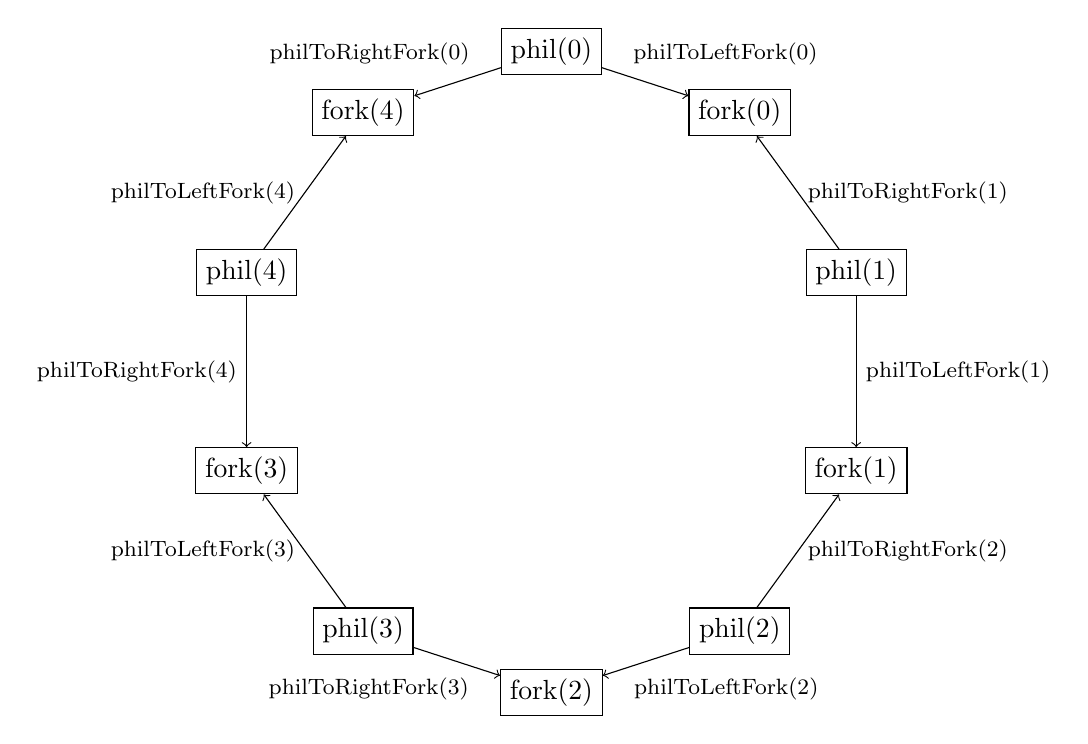
\begin{tikzpicture}
\foreach \i in {0,...,4} 
  \draw (90-72*\i: \r) node[draw] (phil\i) {\scalashape phil(\i)}; 
\foreach \i in {0,...,4} 
  \draw (54-72*\i: \r) node[draw] (fork\i) {\scalashape fork(\i)}; 
%
\draw[->] (phil0) -- node[above right, near start] 
  {\scalashape\footnotesize philToLeftFork(0)} (fork0);
\draw[->] (phil1) -- node[right] 
  {\scalashape\footnotesize philToLeftFork(1)} (fork1);
\draw[->] (phil2) -- node[below right, near end] 
  {\scalashape\footnotesize philToLeftFork(2)} (fork2);
\draw[->] (phil3) -- node[left] 
  {\scalashape\footnotesize philToLeftFork(3)\ } (fork3);
\draw[->] (phil4) -- node[left] 
  {\scalashape\footnotesize philToLeftFork(4)\ } (fork4);
%
\draw[->] (phil0) -- node[above left, near start]
  {\scalashape\footnotesize philToRightFork(0)} (fork4);
\draw[->] (phil1) -- node[right]
  {\scalashape\footnotesize philToRightFork(1)} (fork0);
\draw[->] (phil2) -- node[right]
  {\scalashape\footnotesize philToRightFork(2)} (fork1);
\draw[->] (phil3) -- node[below left, near end]
  {\scalashape\footnotesize philToRightFork(3)} (fork2);
\draw[->] (phil4) -- node[left]
  {\scalashape\footnotesize philToRightFork(4)} (fork3);
\end{tikzpicture}
\end{center}

%%%%%

\begin{scala}
  /** The complete system. */ 
  def system = {
    val philToLeftFork, philToRightFork = Array.fill(N)(new SyncChan[Cmd])
    // £philToLeftFork(i)£ is from £phil(i)£ to £fork(i)£;
    // £philToRightFork(i)£ is from £phil(i)£ to £fork($(\sm i-1) \bmod \sm N$)£.
    val allPhils = || ( 
      for (i <- 0 until N) yield phil(i, philToLeftFork(i), philToRightFork(i))
    )
    val allForks = || ( 
      for (i <- 0 until N) yield
        fork(i, philToRightFork((i+1)%N), philToLeftFork(i))
    )
    allPhils || allForks
  }

  /** Run the system. */
  def main(args : Array[String]) = run(system)
\end{scala}
\caption{The Dining Philosophers example (part 2).}
\label{fig:dining-philosophers-2}
\end{figure}

%%%%%%%%%%%

It is important that we use \emph{synchronous} channels: we need each
philosopher and fork to synchronise on relevant actions. 

\begin{instruction}
Study the details of the implementation.
\end{instruction}

When we run the system, sometimes it deadlocks almost immediately.  A~typical
deadlocking trace is:
%
\begin{scala}
1 sits,  0 sits,  4 sits,  2 sits,  1 picks up left fork, 3 sits,  0 picks up left fork,  
4 picks up left fork, 2 picks up left fork,  3 picks up left fork
\end{scala}
%
Each philosopher sits down and picks up their left fork (in some order).  At
this point, each philosopher is trying to pick up its right fork, i.e.~to send
a |Pick| message on its |right| channel; however, the corresponding fork is
not willing to receive that message.  This means that the system is
deadlocked.

Recall that typing \texttt{Ctrl}+$\backslash$ (control and backslash) produces
a thread dump.  This gives the line number in the code where each thread is
stuck, so can help to understand the deadlock.

However, sometimes when we run the system, it runs for a very long time
without deadlocking.  In fact, I chose the delays in the simulations of the
basic actions so that the system deadlocks about half the time.  Different
choices for these delays would have caused the system to deadlock on nearly
every run, or hardly ever.  In some ways, the latter situation is worse: it is
likely that the potential deadlock would not be found by routine testing, but
that it would occur only when the system is deployed.

%%%%%%%%%%%%%%%%%%%%%%%%%%%%%%%%%%%%%%%%%%%%%%%%%%%%%%%%%%%%%%%%%

\section{Logging and Debugging}

In the above simulation, we used |println| statements so that we could
understand what happened.  However, this style is often not convenient when
tracking down bugs.  Normally, a better way to is to use logging.

The SCL class |Log| provides log objects.
%
A new log storing events of type~|A|, suitable for |p| threads,
can be defined by
\begin{scala}
  val log = new Log[A](p)
\end{scala}
%
This provides operations
%
\begin{itemize}
\item |def add(me: Int, x: A)|, which adds |x| to the log, performed by
  thread~|me|, where $\sm{me} \in \interval{0}{\sm p}$;

\item |def get: Array[A]|, which gets the contents of the log;

\item |def toFile(fname: String = "/tmp/logFile")|, which writes the contents
  of the log to the file~|fname| (with a default of \texttt{/tmp/logFile}).
\end{itemize}

The code in Figure~\ref{fig:dining-phils-log} shows how we can use logging in
the dining philosophers example.  (I have arranged for philosopher~|0| to
print a dot on each iteration, so we can tell whether the system is making
progress.)

%%%%%

\begin{figure}
\begin{scala}
  val log = new Log[String](N)
 
  def phil(me: Int, left: !![Cmd], right: !![Cmd]) = thread(s"Phil $me"){
    repeat{
      think()
      log.add(me, s"$me sits"); pause()
      left!Pick; log.add(me, s"$me picks up left fork"); pause()
      right!Pick; log.add(me, s"$me picks up right fork"); pause()
      log.add(me, s"$me eats"); eat()
      left!Drop; pause(); right!Drop; pause()
      log.add(me, s"$me leaves")
      if(me == 0) print(".")
    }
  }
\end{scala}
\caption{Using a {\scalashape Log} object.}
\label{fig:dining-phils-log}
\end{figure}

%%%%%

In many scenarios, when the system terminates, we can either write the log to
a file, or analyse the log using some code.  However, this won't work when the
system deadlocks.  Instead, we need to insert a hook that will arrange for the
log to write itself to a file when the user interrupts the program.  This can
be done with the |writeToFileOnShutdown| method:
%
\begin{scala}
  def main(args: Array[String]) = {
    log.writeToFileOnShutdown("philsLog.txt"); run(system)
  }
\end{scala}

Logging is a general technique that can help with debugging.  However, there
is a wrinkle concerning its usage.
%
Internally, each thread uses its own thread-local log, to avoid race
conditions, and for efficiency.  This is why the |log| operation takes the
thread's identity as a parameter: different threads should use different
identities, in the relevant range.  Each logged value is stored in the
relevant thread-local log, together with a timestamp (more precisely, the
time elapsed since the |Log| object was created, to avoid problems with
timestamp wrap-around).
%
The |get| operation merges the thread-local logs according to
timestamps.

Using timestamps in this way assumes that the clocks are loosely synchronised
across cores, and that the granularity of the clocks is sufficiently fine, so
that if one |add| event logically happens before another (i.e.~according to
the~$\prec$ relation), the former receives a strictly smaller timestamp.

The above assumption seems to be sound in Linux, but not in Windows.  If you
must use Windows, the class |SharedLog| provides the same interface.  However,
it will give worse performance.  Further, it might affect the likelihood of
detecting bugs: I have experienced bugs that would appear when no logging was
performed, or when the timestamp-based log was used; but logging with
something equivalent to |SharedLog| affected the speed of threads sufficiently
that the bug no longer appeared in a reasonable time!


 % Dining Philosophers
\section{Avoiding Deadlocks}
\label{sec:avoid-deadlocks}

\def\waitingFor{\vdash}

The deadlock in the Dining Philosophers example corresponds to a cycle of
waiting.  Each philosopher is trying to pick up their right-hand fork, and is
waiting for that fork.  Each fork is waiting for their right-hand philosopher
to put it down.  Let's write $t_1 \waitingFor t_2$ to signify that thread
$t_1$ is blocked, waiting for thread~$t_2$.  Then we have the following cycle
of waiting:
\[\mstyle
\sm{phil}(0) \waitingFor \sm{fork}(4) \waitingFor \sm{phil}(4) \waitingFor
  \sm{fork}(3) \waitingFor \ldots \waitingFor \sm{fork}(0) \waitingFor
  \sm{phil}(0).
\]
This corresponds to an anti-clockwise cycle in
Figure~\ref{fig:dining-philosophers-2}.

In fact, deadlocks correspond to cycles of waiting more generally.  Consider a
system based on message passing.  Suppose that for every channel~$c$, there
is some thread that sometimes sends on~$c$, and some thread that sometimes
receives on~$c$ (or else the system is badly configured).  Consider a
deadlocked state, and suppose no thread has terminated or is performing an
infinite amount of internal computation.  Then necessarily every thread is
trying to send or receive on a channel.  Pick a thread $t_1$.  It is trying to
send or receive on some channel~$c_1$, so necessarily there is some
thread~$t_2$ that sometimes receives or sends (respectively) on~$c_1$; hence
$t_1$ is waiting for~$t_2$, i.e.~$t_1 \waitingFor t_2$.  By the same argument,
there is some thread $t_3$ such that $t_2 \waitingFor t_3$.  Continuing in
this way, we can construct an infinite sequence of threads such that each is
waiting on the next.  However, there are necessarily finitely many threads, so
this infinite sequence must contain the same thread twice, and so contains a
waiting cycle.

If the system uses an alt, then a thread may be waiting for either of two or
more threads.  For example, in the dining philosophers example, a fork in its
initial state is waiting for either its left- or right-hand philosopher
(although there is no deadlocked system state corresponding to this state for
the fork).  In such cases, a deadlocked state may contain multiple waiting
cycles, and breaking any one of them would remove the deadlock.  A similar
fact is true when a channel is shared by several receivers, so a sender might
be waiting for any one of those receivers; and similarly when a channel is
shared by several senders.

There are a couple of ways of adapting the dining philosophers example so as
to remove the possibility of deadlock.  Each involves removing the possibility
of a waiting cycle.  Exercise~\ref{ex:diningPhils} asks you to implement
these. 

Note that whenever a philosopher is holding a fork but trying to drop it, that
action is never blocked.  Thus a philosopher that is waiting must be trying to
pick up a fork, but that fork is held by another philosopher.  That fork,
then, is waiting for the latter philosopher to drop it.  And the latter
philosopher must be waiting to pick up the next fork.  Continuing in this way,
we see that any waiting cycle must involve \emph{all} the philosophers and
forks. 

One way to avoid deadlocks is to introduce a ``butler'' thread that ensures
that there are never more than four philosophers seated.  We argue by
contradiction that there is then no deadlocked state.  Suppose otherwise.  Not
all philosophers can be seated, by design.  Without loss of generality,
suppose philosopher~$0$ is not currently seated.  Then necessarily that
philosopher cannot be holding fork~$0$ or fork~$4$.  But this then removes the
possibility of a waiting cycle, because neither of those forks is waiting for
philosopher~$0$.  This contradicts the observation in the previous paragraph
that any waiting cycle most involve all the threads.

In the earlier version of the dining philosophers example, all philosophers
picked up their left fork before their right fork.  Another way to avoid the
deadlock is for some (but not all) of the philosophers to pick up their right
fork first.  If that is the case, there must be an adjacent pair of
philosophers neither of whom picks up their shared fork first.  Without loss
of generality, suppose philosopher~$0$ picks up fork~$4$ before fork~$0$, and
philosopher~$1$ picks up fork~$1$ before fork~$0$.  This then removes the
possibility of a waiting cycle.  If either philosopher~$0$ or philosopher~$1$
holds fork~$0$ then they have necessarily already picked up their other fork,
and so can drop a fork.  Alternatively, if neither philosopher holds fork~$0$,
then that fork cannot be part of a waiting cycle.

Another way to avoid deadlocks is to detect that a potential deadlock has been
reached, and to react to remove that possibility, by backtracking.  For
example, if a philosopher holds one fork, but is unable to pick up their
second fork, they could drop their first fork, and try again later (this is
probably how real philosophers would act).

Within SCL, this could be achieved using a timeout.  Each channel has an
operation
%
\begin{scala}
  def sendWithin(millis: Long)(x: A): Boolean 
\end{scala}
%
This tries to send~|x| for up to |millis| milliseconds; but if no receiver is
ready within that time (or no space is available, in the case of a buffered
channel), it times out.  The operation returns a |Boolean| to indicate whether
the send was successful.  Likewise there is an operation
%
\begin{scala}
  def receiveWithin(millis: Long): Option[A] =
\end{scala}
%
that tries to receive a value for up to |millis| milliseconds.  The operation
returns a result of type |Option[A]| (see Scala box~\ref{sb:option-type}): if it
successfully receives a value~|x|, it returns~|Some(x)|; otherwise it
returns~|None| to indicate a timeout.  There are also operations
|sendWithinNanos| and |receiveWithinNanos| where the time is given in
nanoseconds.

The last part of Exercise~\ref{ex:diningPhils} asks you to implement this
technique of timing out, dropping the fork, and trying again later.

%%%%%%%%%%%%%%%%%%%%%%%%%%%%%%%%%%%%%%%%%%%%%%%%%%%%%%%

\section{Alts with Out-ports}

So far, we have only seen alts that provide a choice between in-ports.
However, it is also possible to use an out-port in an alt, using the following
syntax for a branch:
%
\begin{scala}
  bool && out =!=> { expression }
\end{scala}
%
If the (optional) boolean guard |bool| is true, when the out-port |out| is
ready for communication, |expression| is evaluated and the result sent.
%
Sometimes it's necessary to do something \emph{after} the value has been sent,
using a continuation, with the following syntax.
%
\begin{scala}
   bool && outport =!=> { expression } ==> { command }
\end{scala}

Here's another definition for the |tee| function, which produces
a thread that inputs on one in-port, and outputs on two out-ports, in either
order. 
%
%\begin{mysamepage}
\begin{scala}
  def tee[T](in: ??[T], out1: !![T], out2: !![T]) = thread{
    repeat{ 
      val v = in?()
      alt( out1 =!=> { v } ==> { out2!v } | out2 =!=> { v } ==> { out1!v } )
    }
  }
\end{scala}
%
This sends~|v| on whichever out-port is ready first, and then sends~|v| on the
other out-port.
%\end{mysamepage}

%%%%%% A two-place buffer

In-ports and out-ports can be mixed within an \SCALA{alt}.
%
The following code copies data from |in| to |out|, and can hold up to two
pieces of data at a time: it is a two-place buffer. 
%
\begin{scala}  
  def buff2[T](in: ??[T], out: !![T]): ThreadGroup = {
    def empty(): Unit = { val x = in?(); full(x) }
    def full(x: T): Unit = {
      alt( out =!=> { x } ==> { empty() } | in =?=> { y => out!x; full(y) } )
    }
    thread{ attempt{empty()}{} }
  }
\end{scala}
%%   /** Two place buffer. */
%%   def buff2[T](in: ??[T], out: !![T]): Unit = {
%%     val x = in?(); buff2A(in, out, x)
%%   }
%%   /** Two place buffer holding £x£. */
%%   def buff2A[T](in: ??[T], out: !![T], x: T): Unit = {
%%     alt(
%%       out =!=> { x } ==> { buff2(in, out) }
%%       | in =?=> { y => out!x; buff2A(in, out, y) }
%%     )
%%   }  
%% \end{scala}
%
This runs a thread that executes |empty()|, catching |Stopped| exceptions.
When it  holds a value~|x|, in state |full(x)|, it can either
output~|x|, or input a new value~|y|, at which point it is full so must
output~|x|, after which it is just holding~|y|.


Here's an alternative definition.  The variable \SCALA{empty} records whether
the buffer is empty.  When $\sm{empty} = \sm{false}$,\, \SCALA{x} stores the
next value to be output.
%
%\begin{mysamepage}
\begin{scala}
  def buff2Alt[T](in: ??[T], out: !![T]) = thread{
    var x: T = null.asInstanceOf[T]  // Contents, possibly invalid.
    var empty = true // Is the buffer empty?
    serve(
      !empty && out =!=> { empty = true; x }
      | empty && in =?=> { v => x = v; empty = false }
      | !empty && in =?=> { v => out!x; x = v }
    )
  }
\end{scala}
%\end{mysamepage}
%
\noindent
In the first branch, the code \SCALA{\{ empty = true; x \}} is an expression
whose value is~|x|, but which has the side effect of setting |empty| to |true|. 
The last two branches could be merged, and an \SCALA{if} statement used. 
%
\begin{scala}
    | in =?=> { v => if(empty){ x = v; empty = false } else { out!x; x = v } }
\end{scala}

%% --- Moved to exercise
%% Here's another example, namely a thread that receives data on |in|, and
%% outputs it on |out|.  It acts as a buffer, internally holding data in a
%% |Queue| from the Scala Application Programming Interface.  It is equivalent to
%% an |UnboundedBuffChan| (although the latter doesn't use a separate thread
%% internally).
%% %
%% \begin{scala}
%%   def buffer[A](in: ??[A], out: !![A]) = thread("buffer"){
%%     val q = new scala.collection.mutable.Queue[A]
%%     serve(
%%       in =?=> { x => q.enqueue(x) }
%%       | q.nonEmpty && out =!=> { q.dequeue() }
%%     )
%%     in.close(); out.endOfStream()
%%   }
%% \end{scala}
%% %
%% Note that in the second branch, it is important that the alternation evaluates
%% the expression |q.dequeue()| only \emph{after} another thread has committed to
%% communicating on~|out|: otherwise the dequeued value would be lost if no
%% communication takes place. 

%%%%%%%%%%%%%%%%%%%%%%%%%%%%%%%%%%%%%%%%%%%%%%%%%%%%%%%

As with in-ports, an out-port may not be simultaneously feasible in two
alternations.  Further, both ports of a channel may not simultaneously be
feasible in alternations, i.e.~you can't have one alternation trying to send
on a channel, and another alternation trying to receive on the same channel.
The implementation detects violations of these two restrictions, and throws an
exception.
 % With outports

%%%%%%%%%%%%%%%%%%%%%%%%%%%%%%%%%%%%%%%%%%%%%%%%%%%%%%%%%%%%

\section{Misc}

\begin{slide}
\heading{\protect\SCALA{alt}s versus shared channels}

Sometimes a shared channel can produce the same effect as an \SCALA{alt}.

For example, consider a variant of the dining philosophers where each
philosopher has channels \SCALA{pick} and \SCALA{drop} for each of its
forks, and where each fork has single \SCALA{pick} and \SCALA{drop}
channels, on which it can receive messages from either of the adjacent
philosophers:
%
\begin{scala}
  def Fork(me: Int, pick: ??[Unit], drop: ??[Unit]) = thread("Fork"+me){
    repeat{ pick?(); drop?() }
  }
\end{scala}
%
%% Note that the \SCALA{pick} communication could be from either neighbouring
%% philosopher, so these need to be |ManyOne| channels.
Note that we need separate |pick| and |drop| channels.
\end{slide}

%%%%%


\begin{slide}
\heading{Restrictions}

\begin{itemize}
%% \item
%% An alt may not have two simultaneously enabled branches using the
%% same port.

%% \item An alt may not use a port that is shared, either with another alt or
%% with a non-alt read or write.

\item A port may not be simultaneously feasible in two alts or |serve|s.
  (But it may be feasible in an alt/|serve|, and also used by a thread with
  a simple send or receive.)

\item Both ports of a channel may not simultaneously be feasible in alts or
  |serve|s.
\end{itemize}
%
The implementation  detects violations. 
\end{slide}

%%%%%

\begin{slide}
\heading{Generalised \protect\SCALA{alt}s}

\SCALA{alt}s (and \SCALA{serve}s) can be constructed from collections of
branches.

Here is a generalization of the tagger:
%
\begin{scala}
def tagger[T](ins: List[??[T]], out: !![(Int, T)]) = thread{
  serve ( 
    | (for (i <- 0 until ins.length) yield ins(i) =?=> { x => out!(i, x) })
  )
  for (in <- ins) in.close
  out.endOfStream
}
\end{scala}

This will terminate when all input channels are closed, or \SCALA{out} is
closed. 
\end{slide}

%%%%%

\begin{slide}
\heading{Caveat}

alts and |serve|s are fairly heavyweight constructs.  Don't use them unless
there's a good reason to do so, i.e.~you really want to be able to communicate
on either of two channels.
Sometimes it's easier and more efficient to force communications to happen in
a particular order.
\end{slide}

%%%%%%%%%%%%%%%%%%%%%%%%%%%%%%%%%%%%%%%%%%%%%%%%%%%%%%%%%%%%

\section{Summary}


\begin{itemize}
\item
\SCALA{alt}s;

\item
Syntax: using inports and outports; guards; \SCALA{serve}; generalised alts;
% timeouts; \SCALA{orelse}; \SCALA{prialt} (and \SCALA{priserve})

\item
Example: dining philosophers;

\item
Logging;

%% \item
%% \SCALA{alt}s versus \SCALA{ManyOne} channels;

\item
Restrictions on use of \SCALA{alt}s. 
\end{itemize}


%%%%%%%%%%%%%%%%%%%%%%%%%%%%%%%%%%%%%%%%%%%%%%%%%%%%%%%

\section*{Exercises}

\begin{question}
\label{ex:diningPhils}
The aim of this question is to investigate some variants of the Dining
Philosophers example that aim to avoid deadlocks, as discussed in
Section~\ref{sec:avoid-deadlocks}.  You should implement and test each of the
three variants below.
%
\begin{enumerate}
\item \textbf{A right-handed philosopher.}
In the standard version of the Dining Philosophers, all the philosophers are
left-handed: they pick up their left fork first.  Implement a variant where
one of the philosophers is right-handed, i.e.\ they pick up their right fork
first.

\item \textbf{Using a butler.} Now consider a variant using an extra
  thread, which represents a butler.  The butler makes sure that no more than
  four philosophers are ever simultaneously seated.

\item \textbf{Using timeouts.} Now consider a variant where, if a philosopher
  is unable to obtain their second fork within a reasonable time, they put
  down their first fork and try again later.  In the version in the body of this
  chapter, all delays are a few hundred milliseconds, so the period spent
  attempting to pick up the second fork should be of a similar order.  You
  will need to use the |sendWithin| operation, described earlier.

If the system reaches a state where all philosophers are blocked, it's
possible that they all put down their forks at the same time, and then all
retry at the same time, leading to them being blocked again.  How can we avoid
this happening repeatedly?
\end{enumerate}
\end{question}

%%%%%%%%%%%%%%%%%%%%%%%%%%%%%%%%%%%%%%%%%%%%%%%%%%%%%%%

\begin{answerI}
In the answers below, I'll elide code that is identical to that in the body of
the chapter.

\begin{enumerate}
\item
The following code makes philosopher~$0$ right-handed.
%
\begin{scala}
  def phil(me: Int, left: !![Cmd], right: !![Cmd]) = thread("Phil"+me){
    repeat{
      ... // Thinks, and then sits.
      if(me == 0){
        right!Pick; println(s"$me picks up right fork"); pause()
        left!Pick; println(s"$me picks up left fork"); pause()
      }
      else{
        left!Pick; println(s"$me picks up left fork"); pause()
        right!Pick; println(s"$me picks up right fork"); pause()
      }
      ... // Drops forks, and leaves.
    }
  }
\end{scala}

%%%%%

\item We can use the following channels for a philosopher to signal to the
  butler that they want to sit down or are leaving.
\begin{scala}
  private val sit, leave = new SyncChan[Unit]
\end{scala}
%
The definition of a philosopher is easily adapted to use these channels.%
\begin{scala}
  def phil(me: Int, left: !![Cmd], right: !![Cmd]) = thread("Phil"+me){
    repeat{
      think()
      sit!(); println(s"$me sits"); pause()
      ... // Picks up forks, eats, drops forks.
      leave!(); println(s"$me leaves")
    }
  }
\end{scala}
%
The butler keeps track of how many philosophers are currently seated.  When
there are already $\sm N - 1$ seated, the butler prevents the final
philosopher from sitting down by refusing a communication on |sit|.  As a
sanity-check, the code below checks that, when a philosopher leaves, there was
at least one philosopher previously seated.
%
\begin{scala}
   def butler = thread("butler"){
    var seated = 0 // Number currently seated.
    serve(
      seated < N-1 && sit =?=> { _ => seated += 1 }
      | leave =?=> { _ => assert(seated > 0); seated -= 1 }
    )
  }
\end{scala}
%
The definition of |system| includes |butler| as an additional parallel
component. 

%%%%%

\item
If a philosopher is unable to obtain their second fork, they drop their first
fork, and then wait for a random amount of time before trying again.  This
randomness makes it more likely that the philosophers get out of sync, and so
succeed next time.  
%
\begin{scala}
  /** Time to wait for second fork. */
  private def waitTime = 300+Random.nextInt(200)

  /** Time to wait after failing to get second fork. */
  private def backoffTime = 200+Random.nextInt(800)
\end{scala}

\begin{scala}
  def phil(me: Int, left: !![Cmd], right: !![Cmd]) = thread("Phil"+me){
    repeat{
      ... // Thinks, and then sits. 
      var done = false
      while(!done){
        left!Pick; println(s"$me picks up left fork"); pause()
        if(right.sendWithin(waitTime)(Pick)){
          println(s"$me picks up right fork"); pause()
          println(s"$me eats"); eat()
          left!Drop; pause(); right!Drop; pause()
          println(s"$me leaves"); done = true
        }
        else{
          println(s"$me fails to get right fork"); pause()
          left!Drop; Thread.sleep(backoffTime)
        }
      } // End of £while£ loop.
    }
  }
\end{scala}
\end{enumerate}
\end{answerI}

 % DP practical

Adaptive quadrature 
